\documentclass[10pt, aspectratio=169]{beamer}

\usepackage[T1]{fontenc}
\usepackage[utf8]{inputenc}
\usepackage[slovene]{babel}
\usepackage{lmodern}
\usepackage{amsfonts,amssymb,amsmath}
\usepackage{pgfpages}
% \usepackage{tikz}
\usepackage{wrapfig}
\usepackage{graphicx}
\usepackage{pgfkeys}
\usepackage{pgfplots}
\usepackage{xcolor}
\usepackage{tkz-euclide}
\usepackage{xfp}
% \usepackage{pgf}

\usetikzlibrary{angles,arrows,arrows.meta,calc,decorations,decorations.markings,decorations.pathreplacing,decorations.shapes,decorations.text,
	decorations.pathmorphing,intersections,math,plotmarks,positioning,quotes,shapes.misc,through}


\setbeameroption{show notes on second screen}
% \setbeameroption{show only notes}

% \usetheme[sectionpage=simple, titlestyle=plain, sectionstyle=style2, slidestyle=style1, numbering=counter, block=fill, headingcolor=theme]{trigon}

\usetheme{CambridgeUS}
\usecolortheme{beaver}



\setbeamerfont{subtitle}{size=\small}


\title{MATEMATIKA}
\subtitle{1. letnik - splošna gimnazija}
\date{\today}
\author{Jan Kastelic}
\institute[FMF]{Fakulteta za matematiko in fiziko, \\ Univerza v Ljubljani}

\newtheorem{izrek}{Izrek}
\newcommand{\Vir}[1]{\color{gray}{\tiny{Vir: #1}}}


\begin{document}

\begin{frame}
	\titlepage
\end{frame}
	
% \titleframe

\begin{frame}
	\frametitle{Vsebina}
	\tableofcontents[hideallsubsections]
\end{frame}
	
\section{Naravna in cela števila}

\begin{frame}
    \sectionpage
\end{frame}

\begin{frame}
    \tableofcontents[currentsection, hideothersubsections]
\end{frame}
        
    \subsection{Naravna števila}

        \begin{frame}
            \frametitle{Naravna števila}

                \only<2->{\begin{alertblock}{Množica naravnih števil}
                    \only<3->{\textbf{Naravna števila} so števila s katerimi štejemo.}
                    \only<4->{$$\mathbf{\mathbb{N}=\{1, 2, 3, 4, \ldots\}}$$}
                \end{alertblock}}

                \only<5->{\begin{block}{}
                    Množico naravnih števil definirajo \textbf{Peanovi aksiomi}:
                    \begin{enumerate}
                        \item<6-> Vsako naravno število $n$ ima svojega \textbf{naslednika} $n+1$.
                        \item<7-> Število $1$ je naravno število, ki ni naslednik nobenega naravnega števila.
                        \item<8-> Različni naravni števili imata različna naslednika: $n+1 \neq m+1; n \neq m$.
                        \item<9-> Če neka trditev velja z vsakim naravnim številom tudi za njegovega naslednika, velja za vsa naravna števila. (\textit{aksiom/princip popolne indukcije})
                    \end{enumerate}

                \end{block}}
        \end{frame}

        \begin{frame}

            \only<2->{\begin{block}{}
                Naravna števila uredimo po velikosti in predstavimo s \textbf{točko} na \textbf{številski premici}.
                \only<3->{\begin{figure}
                    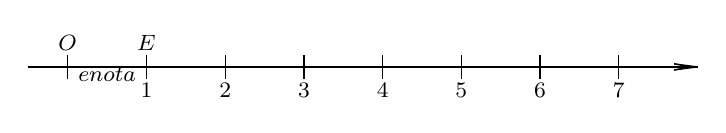
\begin{tikzpicture}
                        % \clip (0,0) rectangle (14.000000,10.000000);
                        {\footnotesize
                        
                        % Drawing segment a b
                        \draw [line width=0.016cm] (0.500000,0.500000) -- (9.000000,0.500000);%
                        
                        % Drawing arrow a b 1.00
                        \draw [line width=0.016cm] (8.702567,0.539158) -- (9.000000,0.500000);%
                        \draw [line width=0.016cm] (8.702567,0.539158) -- (8.900856,0.500000);%
                        \draw [line width=0.016cm] (8.702567,0.460842) -- (9.000000,0.500000);%
                        \draw [line width=0.016cm] (8.702567,0.460842) -- (8.900856,0.500000);%
                        
                        % Drawing segment c d
                        \draw [line width=0.016cm] (1.000000,0.350000) -- (1.000000,0.650000);%
                        
                        % Drawing segment e f
                        \draw [line width=0.016cm] (2.000000,0.350000) -- (2.000000,0.650000);%
                        
                        % Drawing segment g h
                        \draw [line width=0.016cm] (3.000000,0.350000) -- (3.000000,0.650000);%
                        
                        % Drawing segment i j
                        \draw [line width=0.016cm] (4.000000,0.350000) -- (4.000000,0.650000);%
                        
                        % Drawing segment k l
                        \draw [line width=0.016cm] (5.000000,0.350000) -- (5.000000,0.650000);%
                        
                        % Drawing segment m n
                        \draw [line width=0.016cm] (6.000000,0.350000) -- (6.000000,0.650000);%
                        
                        % Drawing segment o p
                        \draw [line width=0.016cm] (7.000000,0.350000) -- (7.000000,0.650000);%
                        
                        % Drawing segment r s
                        \draw [line width=0.016cm] (8.000000,0.350000) -- (8.000000,0.650000);%
                        
                        % Marking point O
                        \draw (1.000000,0.600000) node [anchor=south] { $O$ };%
                        
                        % Marking point E
                        \draw (2.000000,0.600000) node [anchor=south] { $E$ };%
                        
                        % Marking point 1
                        \draw (2.000000,0.400000) node [anchor=north] { $1$ };%
                        
                        % Marking point 2
                        \draw (3.000000,0.400000) node [anchor=north] { $2$ };%
                        
                        % Marking point 3
                        \draw (4.000000,0.400000) node [anchor=north] { $3$ };%
                        
                        % Marking point 4
                        \draw (5.000000,0.400000) node [anchor=north] { $4$ };%
                        
                        % Marking point 5
                        \draw (6.000000,0.400000) node [anchor=north] { $5$ };%
                        
                        % Marking point 6
                        \draw (7.000000,0.400000) node [anchor=north] { $6$ };%
                        
                        % Marking point 7
                        \draw (8.000000,0.400000) node [anchor=north] { $7$ };%
                        
                        % Marking point {enota}
                        \draw (1.500000,0.600000) node [anchor=north] { ${enota}$ };%
                        }
                    \end{tikzpicture}
                        
                \end{figure}}

            \end{block}}

            \only<4->{\begin{block}{}
                Vsako število zapišemo s \textbf{številko}. 
                Za zapis številke uporabljamo \textbf{števke}. Te so $0, 1, 2, 3, 4, 5, 6, 7, 8, 9$.
            \end{block}}

            \only<5->{\begin{block}{}
                Posamezne števke večmestnega števila od desne proti levi predstavljajo: \textbf{enice}, \textbf{desetice}, \textbf{stotice}, \textbf{tisočice}, ...
            \end{block}}

            \only<6->{\begin{block}{}
                Število, ki je zapisano s črkovnimi oznakami števk označimo s črto nad zapsiom črkovne oznake.
                \only<7->{$$ \overline{xy}=10x+y \quad \quad \quad \overline{xyz}=100x+10y+z$$}
            \end{block}}

            
        \end{frame}

        \begin{frame}
            \frametitle{Operacije v množici $\mathbb{N}$}

            \only<2->{\begin{alertblock}{Seštevanje}
                \only<3->{Poljubnima naravnima številoma $x$ in $y$ priredimo \textbf{vsoto} $\mathbf{x+y}$.}
            \end{alertblock}}

            \only<4->{\begin{block}{}
                Število $x$ oziroma $y$ imenujemo \textbf{seštevanec} ali \textbf{sumand} ali \textbf{člen}. 

                \only<5->{Število $x+y$ pa imenujemo \textbf{vsota} ali \textbf{summa}. }

            \only<6->{\begin{figure}
                \begin{tikzpicture}
                    % \clip (0,0) rectangle (14.000000,10.000000);
                    {\footnotesize
                    
                    % Drawing segment a b
                    \draw [line width=0.016cm] (5.000000,0.500000) -- (5.000000,2.500000);%
                    
                    % Drawing segment b d
                    \draw [line width=0.016cm] (5.000000,2.500000) -- (7.000000,2.500000);%
                    
                    % Drawing segment c d
                    \draw [line width=0.016cm] (7.000000,0.500000) -- (7.000000,2.500000);%
                    
                    % Drawing segment c a
                    \draw [line width=0.016cm] (7.000000,0.500000) -- (5.000000,0.500000);%
                    
                    % Drawing segment e f
                    \draw [line width=0.016cm] (7.000000,1.500000) -- (9.000000,1.500000);%
                    
                    % Drawing arrow e f 1.00
                    \draw [line width=0.016cm] (8.702567,1.539158) -- (9.000000,1.500000);%
                    \draw [line width=0.016cm] (8.702567,1.539158) -- (8.900856,1.500000);%
                    \draw [line width=0.016cm] (8.702567,1.460842) -- (9.000000,1.500000);%
                    \draw [line width=0.016cm] (8.702567,1.460842) -- (8.900856,1.500000);%
                    
                    % Drawing segment g h
                    \draw [line width=0.016cm] (2.500000,1.000000) -- (5.000000,1.000000);%
                    
                    % Drawing segment i j
                    \draw [line width=0.016cm] (2.500000,2.000000) -- (5.000000,2.000000);%
                    
                    % Drawing arrow g h 1.00
                    \draw [line width=0.016cm] (4.702567,1.039158) -- (5.000000,1.000000);%
                    \draw [line width=0.016cm] (4.702567,1.039158) -- (4.900856,1.000000);%
                    \draw [line width=0.016cm] (4.702567,0.960842) -- (5.000000,1.000000);%
                    \draw [line width=0.016cm] (4.702567,0.960842) -- (4.900856,1.000000);%
                    
                    % Drawing arrow i j 1.00
                    \draw [line width=0.016cm] (4.702567,2.039158) -- (5.000000,2.000000);%
                    \draw [line width=0.016cm] (4.702567,2.039158) -- (4.900856,2.000000);%
                    \draw [line width=0.016cm] (4.702567,1.960842) -- (5.000000,2.000000);%
                    \draw [line width=0.016cm] (4.702567,1.960842) -- (4.900856,2.000000);%
                    
                    % Marking point {vsota}
                    \draw (8.000000,1.500000) node [anchor=south] { ${vsota}$ };%
                    
                    % Marking point {summa}
                    \draw (8.000000,1.500000) node [anchor=north] { ${summa}$ };%
                    
                    % Marking point {se�tevanec}
                    \draw (3.750000,1.000000) node [anchor=south] { ${seštevanec}$ };%
                    
                    % Marking point {sumand}
                    \draw (3.750000,1.000000) node [anchor=north] { ${sumand}$ };%
                    
                    % Marking point {se�tevanec}
                    \draw (3.750000,2.000000) node [anchor=south] { ${seštevanec}$ };%
                    
                    % Marking point {sumand}
                    \draw (3.750000,2.000000) node [anchor=north] { ${sumand}$ };%
                    
                    % Drawing segment x y
                    \draw [line width=0.032cm] (6.000000,1.000000) -- (6.000000,2.000000);%
                    
                    % Drawing segment z w
                    \draw [line width=0.032cm] (5.500000,1.500000) -- (6.500000,1.500000);%
                    }
                    \end{tikzpicture}
                    
            \end{figure}}


            \end{block}}


            \only<7->{\begin{block}{}
                Vsota naravnih števil je naravno število: $x, y \in \mathbb{N} \Rightarrow x+y \in \mathbb{N}$.

            \end{block}}

        \end{frame}

        \begin{frame}
            \only<2->{\begin{alertblock}{Množenje}
                \only<3->{Poljubnima naravnima številoma $x$ in $y$ priredimo \textbf{produkt} $\mathbf{x\cdot y}$.}
            \end{alertblock}}

            \only<4->{\begin{block}{}
                Število $x$ oziroma $y$ imenujemo \textbf{množenec} ali \textbf{faktor}. 

                \only<5->{Število $x\cdot y$ pa imenujemo \textbf{zmnožek} ali \textbf{produkt}. }

                \only<6->{\begin{figure}
                \begin{tikzpicture}
                    % \clip (0,0) rectangle (14.000000,10.000000);
                    {\footnotesize
                    
                    % Drawing segment a b
                    \draw [line width=0.016cm] (5.000000,0.500000) -- (5.000000,2.500000);%
                    
                    % Drawing segment b d
                    \draw [line width=0.016cm] (5.000000,2.500000) -- (7.000000,2.500000);%
                    
                    % Drawing segment c d
                    \draw [line width=0.016cm] (7.000000,0.500000) -- (7.000000,2.500000);%
                    
                    % Drawing segment c a
                    \draw [line width=0.016cm] (7.000000,0.500000) -- (5.000000,0.500000);%
                    
                    % Drawing segment e f
                    \draw [line width=0.016cm] (7.000000,1.500000) -- (9.000000,1.500000);%
                    
                    % Drawing arrow e f 1.00
                    \draw [line width=0.016cm] (8.702567,1.539158) -- (9.000000,1.500000);%
                    \draw [line width=0.016cm] (8.702567,1.539158) -- (8.900856,1.500000);%
                    \draw [line width=0.016cm] (8.702567,1.460842) -- (9.000000,1.500000);%
                    \draw [line width=0.016cm] (8.702567,1.460842) -- (8.900856,1.500000);%
                    
                    % Drawing segment g h
                    \draw [line width=0.016cm] (2.500000,1.000000) -- (5.000000,1.000000);%
                    
                    % Drawing segment i j
                    \draw [line width=0.016cm] (2.500000,2.000000) -- (5.000000,2.000000);%
                    
                    % Drawing arrow g h 1.00
                    \draw [line width=0.016cm] (4.702567,1.039158) -- (5.000000,1.000000);%
                    \draw [line width=0.016cm] (4.702567,1.039158) -- (4.900856,1.000000);%
                    \draw [line width=0.016cm] (4.702567,0.960842) -- (5.000000,1.000000);%
                    \draw [line width=0.016cm] (4.702567,0.960842) -- (4.900856,1.000000);%
                    
                    % Drawing arrow i j 1.00
                    \draw [line width=0.016cm] (4.702567,2.039158) -- (5.000000,2.000000);%
                    \draw [line width=0.016cm] (4.702567,2.039158) -- (4.900856,2.000000);%
                    \draw [line width=0.016cm] (4.702567,1.960842) -- (5.000000,2.000000);%
                    \draw [line width=0.016cm] (4.702567,1.960842) -- (4.900856,2.000000);%
                    
                    % Marking point {zmno�ek}
                    \draw (8.000000,1.500000) node [anchor=south] { ${zmnožek}$ };%
                    
                    % Marking point {produkt}
                    \draw (8.000000,1.500000) node [anchor=north] { ${produkt}$ };%
                    
                    % Marking point {mno�enec}
                    \draw (3.750000,1.000000) node [anchor=south] { ${množenec}$ };%
                    
                    % Marking point {faktor}
                    \draw (3.750000,1.000000) node [anchor=north] { ${faktor}$ };%
                    
                    % Marking point {mno�enec}
                    \draw (3.750000,2.000000) node [anchor=south] { ${množenec}$ };%
                    
                    % Marking point {faktor}
                    \draw (3.750000,2.000000) node [anchor=north] { ${faktor}$ };%
                    
                    % Drawing circle k
                    \draw [line width=0.016cm] (6.000000,1.500000) circle (0.100000);%
                    
                    % Filling circle k
                    \fill (6.000000,1.500000) circle (0.100000);%
                    }
                    \end{tikzpicture}
                    
            \end{figure}}

            \end{block}}


            \only<7->{\begin{block}{}
                Produkt naravnih števil je naravno število: $x, y \in \mathbb{N} \Rightarrow x\cdot y \in \mathbb{N}$.
            \end{block}}

            \only<8->{\begin{block}{}
                Število $\mathbf{1}$ je \textbf{nevtralni element} za mmnoženje: $1\cdot x = x$.
            \end{block}}

        \end{frame}

        \begin{frame}
            

            \only<2->{\begin{alertblock}{Odštevanje}
                \only<3->{Številoma $x$ in $y$, pri čemer je $x$ večje od $y$ ($x>y$), priredimo \textbf{razliko} $\mathbf{x-y}$.}
            \end{alertblock}}

            \only<4->{\begin{block}{}
                Število $x$ imenujemo \textbf{zmanjševanec} ali \textbf{minuend}, število $y$  pa imenujemo \textbf{odštevanec} ali \textbf{subtrahend}. 

                \only<5->{Številu $x-y$ rečemo \textbf{razlika} ali \textbf{diferenca}. }

                \only<6->{\begin{figure}
                    \begin{tikzpicture}
                        % \clip (0,0) rectangle (14.000000,10.000000);
                        {\footnotesize
                        
                        % Drawing segment a b
                        \draw [line width=0.016cm] (5.000000,0.500000) -- (5.000000,2.500000);%
                        
                        % Drawing segment b d
                        \draw [line width=0.016cm] (5.000000,2.500000) -- (7.000000,2.500000);%
                        
                        % Drawing segment c d
                        \draw [line width=0.016cm] (7.000000,0.500000) -- (7.000000,2.500000);%
                        
                        % Drawing segment c a
                        \draw [line width=0.016cm] (7.000000,0.500000) -- (5.000000,0.500000);%
                        
                        % Drawing segment e f
                        \draw [line width=0.016cm] (7.000000,1.500000) -- (9.000000,1.500000);%
                        
                        % Drawing arrow e f 1.00
                        \draw [line width=0.016cm] (8.702567,1.539158) -- (9.000000,1.500000);%
                        \draw [line width=0.016cm] (8.702567,1.539158) -- (8.900856,1.500000);%
                        \draw [line width=0.016cm] (8.702567,1.460842) -- (9.000000,1.500000);%
                        \draw [line width=0.016cm] (8.702567,1.460842) -- (8.900856,1.500000);%
                        
                        % Drawing segment g h
                        \draw [line width=0.016cm] (2.500000,1.000000) -- (5.000000,1.000000);%
                        
                        % Drawing segment i j
                        \draw [line width=0.016cm] (2.500000,2.000000) -- (5.000000,2.000000);%
                        
                        % Drawing arrow g h 1.00
                        \draw [line width=0.016cm] (4.702567,1.039158) -- (5.000000,1.000000);%
                        \draw [line width=0.016cm] (4.702567,1.039158) -- (4.900856,1.000000);%
                        \draw [line width=0.016cm] (4.702567,0.960842) -- (5.000000,1.000000);%
                        \draw [line width=0.016cm] (4.702567,0.960842) -- (4.900856,1.000000);%
                        
                        % Drawing arrow i j 1.00
                        \draw [line width=0.016cm] (4.702567,2.039158) -- (5.000000,2.000000);%
                        \draw [line width=0.016cm] (4.702567,2.039158) -- (4.900856,2.000000);%
                        \draw [line width=0.016cm] (4.702567,1.960842) -- (5.000000,2.000000);%
                        \draw [line width=0.016cm] (4.702567,1.960842) -- (4.900856,2.000000);%
                        
                        % Marking point {razlika}
                        \draw (8.000000,1.500000) node [anchor=south] { ${razlika}$ };%
                        
                        % Marking point {diferenca}
                        \draw (8.000000,1.500000) node [anchor=north] { ${diferenca}$ };%
                        
                        % Marking point {od�tevanec}
                        \draw (3.750000,1.000000) node [anchor=south] { ${odštevanec}$ };%
                        
                        % Marking point {subtrahend}
                        \draw (3.750000,1.000000) node [anchor=north] { ${subtrahend}$ };%
                        
                        % Marking point {zmanj�evanec}
                        \draw (3.750000,2.000000) node [anchor=south] { ${zmanjševanec}$ };%
                        
                        % Marking point {minuend}
                        \draw (3.750000,2.000000) node [anchor=north] { ${minuend}$ };%
                        
                        % Drawing segment z w
                        \draw [line width=0.032cm] (5.500000,1.500000) -- (6.500000,1.500000);%
                        }
                        \end{tikzpicture}
                        
            \end{figure}}
        \end{block}}

            \only<7->{\begin{block}{}
                Razlika je število, ki ga moramo prišteti številu $y$, da dobimo število $x$.
                \only<8->{$$ (x-y)+y=x $$}
            \end{block}}

        \end{frame}

        \begin{frame}
            \only<2->{\begin{block}{}
                Seštevanje in množenje sta \textit{dvočleni notranji operaciji} v množici naravnih števil $\mathbb{N}$.

                \only<3->{Odštevanje pa ni notranja operacija v množici naravnih števil $\mathbb{N}$.}
            \end{block}}

            \only<4->{\begin{block}{Vrstni red operacij}
                \only<5->{Prednost pri računanju imajo \textbf{oklepaji} (najprej najbolj notranji),} 
                \only<6->{nato sledi \textbf{množenje},}
                \only<7->{na koncu pa imamo še \textbf{seštevanje} in \textbf{odštevanje}.}
            \end{block}}

            \only<8->{\begin{block}{}
                Kadar v izrazu nastopajo enakovredne računske operacije, računamo od leve proti desni.
            \end{block}}

            \only<9->{\begin{block}{}
                Pri množenju količin, ki so označene s črkovnimi oznakami, piko, ki označuje operacijo množenja ponavadi opustimo.
                \only<10->{$$ x\cdot y = xy$$}
            \end{block}}


        \end{frame}

        \begin{frame}
            \frametitle{Osnovni računski zakoni v $\mathbb{N}$}

            \only<2->{\begin{block}{Komutativnost seštevanja -- zakon o zamenjavi členov}
                \only<3->{$$ \mathbf{x+y=y+x}$$}
                \only<4->{Vsota ni odvisna od vrstnega reda seštevanja.}
            \end{block}}

            \only<5->{\begin{block}{Asociativnost seštevanja -- zakon o poljubnem združevanju členov}
                \only<6->{$$ \mathbf{(x+y)+z=x+(y+z)}$$}
                \only<7->{Vsota več kot dveh sumandov ni odvisna od združevanja po dveh sumandov.}
            \end{block}}

        \end{frame}

        \begin{frame}


            \only<2->{\begin{block}{Komutativnost množenja -- zakon o zamenjavi faktorjev}
                \only<3->{$$ \mathbf{x\cdot y=y\cdot x}$$}
                \only<4->{Produkt ni odvisen od vrstnega reda faktorjev.}
            \end{block}}

            \only<5->{\begin{block}{Asociativnost množenja -- zakon o poljubnem združevanju faktorjev}
                \only<6->{$$ \mathbf{(x\cdot y)\cdot z=x\cdot (y\cdot z)}$$}
                \only<7->{Produkt več kot dveh sumandov ni odvisen od združevanja faktorjev.}
            \end{block}}

            \only<8->{\begin{block}{Distributivnost -- zakon o razčlenjevanju}
                \only<9->{$$ \mathbf{x\cdot z+y\cdot z = (x+y)\cdot z} $$}
                \only<10->{Če to beremo iz desne proti levi, rečemu tudi \textit{pravilo izpostavljanja skupnega faktorja}.}
            \end{block}}

        \end{frame}

        \begin{frame}
            \only<2->{\begin{exampleblock}{Naloga}
                Izračunajte.
                \only<3->{\begin{itemize}
                    \item $(1+2\cdot 7)+3\cdot(2\cdot 2+7)$ \\ ~
                    \item $3\cdot(2+3\cdot 5)\cdot(2+1)$ \\ ~
                    \item $7+(2+6\cdot 3)+(8+4\cdot 5)$ \\ ~
                    \item $11\cdot 4+(12-6)\cdot 5$ \\ ~
                    \item $8+2\cdot(3+7)-15$ \\ ~
                    \item $37-5\cdot(10-3)$ \\ ~
                \end{itemize}}
            \end{exampleblock}}
        \end{frame}

        \begin{frame}
            \only<2->{\begin{exampleblock}{Naloga}
                Hitro izračunajte.
                \only<3->{\begin{itemize}
                    \item $45+37+15$ 
                    \item $108+46-28$
                    \item $5\cdot 13\cdot 8$
                    \item $4\cdot 7\cdot 25$
                    \item $(7+3)\cdot 2\cdot 5$
                    \item $15\cdot(4+6)\cdot 2$
                    \item $3\cdot 5+7\cdot 5$
                    \item $8\cdot 12+6\cdot 8$
                \end{itemize}}
            \end{exampleblock}}
        \end{frame}

        \begin{frame}
            \only<2->{\begin{exampleblock}{Naloga}
                Zapišite račun glede na besedilo in izračunajte.
                \only<3->{\begin{itemize}
                    \item Produktu števil $12$ in $27$ odštejte razliko števil $19$ in $11$. \\ ~
                    \item Vsoti produkta $4$ in $12$ ter produkta $5$ in $16$ odštejte $8$. \\ ~
                    \item Vsoto števil $42$ in $23$ pomnožite z razliko števil $58$ in $29$. \\ ~
                    \item Produkt števil $14$ in $17$ pomnožite z vsoto števil $5$ in $16$. \\ ~ \\ ~
                \end{itemize}}
            \end{exampleblock}}
        \end{frame}

        \begin{frame}
            \only<2->{\begin{exampleblock}{Naloga}
                Rešite besedilno nalogo.
                \only<3->{\begin{itemize}
                    \item V trgovini kupimo tri litre mleka in štiri čokoladne pudinge v prahu. Če stane liter mleka $95$ centov,
                        čokoladni puding v prahu pa $24$ centov, koliko moramo plačati? \\ ~ \\ ~ \\ ~ \\ ~
                    \item Manca bo kuhala rižoto za štiri otroke in šest odraslih. Za otroško porcijo rižote zadošča $45~g$ riža,
                        za odraslo pa $75~g$. Koliko riža mora dati kuhati za rižoto? \\ ~ \\ ~ \\ ~ \\ ~
                \end{itemize}}
            \end{exampleblock}}
        \end{frame}

\subsection{Cela Števila}
        \begin{frame}
            \frametitle{Cela števila}

                \only<2->{\begin{alertblock}{Množica celih števil}
                    \only<3->{$$\mathbf{\mathbb{Z} = \{\ldots, -2, -1, 0, 1, 2, 3, \ldots\}}$$}
                \end{alertblock}}

                \only<4->{\begin{block}{}
                    Množica celih števil $\mathbb{Z}$ je definirana kot unija treh množic:
                        \begin{itemize}
                            \item<5-> množica \textbf{pozitivnih celih števil} ($\mathbb{Z}^+$) -- naravna števila $\mathbb{N}$;
                            \item<6-> \textbf{število 0};
                            \item<7-> množica \textbf{negativnih celih števil} ($\mathbb{Z}^-$) -- nasprotna števila vseh naravnih števil.
                        \end{itemize}
                      \only<8->{$$\mathbb{Z} = \mathbb{Z}^- \cup \{0\} \cup \mathbb{Z}^+$$}

                \end{block}}

                \only<9->{\begin{block}{}
                    \textbf{Nasprotna vrednost} števila $n$ je število $-n$.
                \end{block}}
        \end{frame}

        \begin{frame}
            \frametitle{Operacije v množici $\mathbb{Z}$}

            \only<2->{\textbf{\large{Seštevanje}}}

            \only<3->{\begin{block}{}
                $$\mathbf{x+0=x}; ~\forall x\in\mathbb{Z}$$
                \only<4->{Število $0$ je \textbf{nevtralni element} pri seštevanju.}
            \end{block}}

            \only<5->{\begin{block}{}
                $$\mathbf{x+(-x)=0}; ~\forall x\in\mathbb{Z} $$
                \only<6->{Vsota celega števila in njemu nasprotnega števila je enaka $0$.}
            \end{block}}

            \only<7->{\begin{block}{}
                $$\mathbf{-(-x)=x}; ~\forall x\in\mathbb{Z}$$
                \only<8->{Nasprotna vrednost nasprotne vrednosti je enaka prvotni vrednosti.}
            \end{block}}
        \end{frame}


        \begin{frame}

            \only<2->{\begin{block}{}
                Vsota dveh pozitivnih števil je pozitivno število, vsota dveh negativnih števil pa je negativno število.
            \end{block}}

            \only<3->{\begin{block}{}
                $$\mathbf{-x+(-y)=-(x+y)}$$
                \only<4->{Vsota nasprotnih vrednosti je enaka nasprotni vrednosti vsote.}
            \end{block}}

            \only<5->{\begin{block}{}
                Naj bosta $x$ in $y$ naravni števili. Vsota pozitivnega števila $x$ in negativnega števila $-y$ je:
                \begin{itemize}
                    \item<6-> pozitivno število, če je $x>y$ in
                    \item<7-> negativno število, če je $x<y$.
                \end{itemize}
            \end{block}}
        \end{frame}


        \begin{frame}
            \only<2->{\textbf{\large{Odštevanje}}}

            \only<3->{\begin{block}{}
                Razlika $x-y$ dveh pozitivnih števil $x$ in $y$ je:
                \begin{itemize}
                    \item<4-> pozitivno število, če je $x>y$ in 
                    \item<5-> negativno število, če je $x<y$.
                \end{itemize}
            \end{block}}

            \only<6->{\begin{block}{}
                Razlika dveh negativnih števil $(-x)-(-y)$ je:
                \begin{itemize}
                    \item<7-> pozitvno število, če je $x<y$ in 
                    \item<8-> negativno število, če je $x>y$.
                \end{itemize}
            \end{block}}

            \only<9->{\begin{block}{}
                Razlika pozitivnega števila $x$ in negativnega števila $-y$ je pozitvno število.
            \end{block}}


            \only<10->{\begin{alertblock}{}
                \textit{Odštevanje v množici $\mathbb{Z}$ je prištevanje nasprotne vrednosti.}
                \only<11->{$$\mathbf{x-y=x+(-y)} $$}
            \end{alertblock}}
        \end{frame}

        \begin{frame}
            \only<2->{\textbf{\large{Množenje}}}

            \only<3->{\begin{block}{}
                $$\mathbf{1\cdot x=x}; ~\forall x\in\mathbb{Z}$$
                \only<4->{Število $1$ je \textbf{nevtralni element} za množenje.}
            \end{block}}

            \only<5->{\begin{block}{}
                $$\mathbf{(-1)\cdot x=-x}; ~\forall x\in\mathbb{Z}$$
                \only<6->{Pri množenju celega števila $x$ z $-1$ dobimo nasprotno število $-x$.}
            \end{block}}

            \only<7->{\begin{block}{}
                $$\mathbf{0\cdot x=0}; ~\forall x\in\mathbb{Z}$$
                \only<8->{Rezultat množenja števila s številom $0$ je enak $0$.}
            \end{block}}

        \end{frame}

        \begin{frame}


            \only<2->{\begin{block}{}
                $$\mathbf{(-x)(-y)=xy}$$
                \only<3->{Produkt sodo mnogo negativnih števil je pozitivno število.}
            \end{block}}

            \only<4->{\begin{block}{}
                $$\mathbf{-x\cdot y=-(xy)}$$
                \only<5->{$$\mathbf{x(-y)=-(xy)}$$}
                \only<6->{Produkt pozitivnega in negativnega števila je negativno število.}
            \end{block}}

            \only<7->{\begin{block}{}
                $$\mathbf{(-x)(-y)=xy}$$
                \only<8->{Produkt liho mnogo negativnih faktorjev je negativno število.}
            \end{block}}

            \only<9->{\begin{block}{}
                Seštevanje, odštevanje in množenje so v množici $\mathbb{Z}$ dvočlene notranje operacije.
            \end{block}}
        \end{frame}


        \begin{frame}
            \frametitle{Osnovni računski zakoni v $\mathbb{Z}$}


        \end{frame}

    %     \begin{frame}

    %         Poleg seštevanja in množenja je kot notranja operacija množice celih števil
    %         definirano še \textbf{odštevanje}.

    %         Za odštevanje velja zakon \textit{\textbf{distributivnosti}}: $a \cdot (b-c) = a \cdot b - a
    %         \cdot c$.

    %     \end{frame}

    %     \begin{frame}
    %         \textbf{\large{Računski zakoni}}

    %         \smallskip
    %         \begin{itemize}
    %             \item Komutativnostni zakon: $$a+b = b+a ~\text{in}~ a \cdot b = b \cdot a$$
    %             \item Asociativnostni zakon: $$a+(b+c) = (a+b)+c ~\text{in}~ a \cdot (b \cdot c) = (a \cdot b) \cdot c$$
    %             \item Zakon o nevtralnem elementu: $$a+0 = a ~\text{in}~ a \cdot 1 = a$$
    %             \item Zakon o inverznem/nasprotnem elementu: $$a+(-a) = 0$$
    %             \item Distributivnostni zakon: $$a \cdot (b \pm c) = a \cdot b \pm a \cdot c$$
    %         \end{itemize}


    %     \end{frame}

    %     \begin{frame}
    %         \textbf{\large{Pravila za računanje s celimi števili}}

    %         \bigskip
    %         \begin{itemize}
    %             \item $-(-a)=a$
    %             \item $0\cdot a=0$
    %             \item $-1 \cdot a =-a$
    %             \item $(-a)+(-b)=-(a+b)$
    %             \item $(-a)\cdot b=-(a\cdot b)=a\cdot (-b)$
    %             \item $(-a)\cdot(-b)=a\cdot b$
    %         \end{itemize}
    %     \end{frame}

    %     \begin{frame}

    %     \end{frame}


    % \subsection{Računanje z naravnimi in celimi števili}

    %     \begin{frame}
    %         \frametitle{Računanje z naravnimi in celimi števili}
    %     \end{frame}

    % \subsection{Izraz, enačba, neenačba}

    %     \begin{frame}
    %         \frametitle{Izraz, enačba, neenačba}
    %     \end{frame}

        % \begin{frame}
        %     \frametitle{Neenačba}

        %     \begin{alertblock}{Neenačba}
        %         Neenačba je zapis, v katerem sta dva izraza v ustrezni relaciji.

        %             $$\left\langle \textmd{izraz_1}\right\rangle < \left\langle \textmd{izraz_2}\right\rangle $$
        %             $$\left\langle \textmd{izraz_1}\right\rangle \leq \left\langle \textmd{izraz_2}\right\rangle $$ 
        %             $$\left\langle \textmd{izraz_1}\right\rangle > \left\langle \textmd{izraz_2}\right\rangle $$ 
        %             $$\left\langle \textmd{izraz_1}\right\rangle \geq \left\langle \textmd{izraz_2}\right\rangle $$  

        %     \end{alertblock}
        % \end{frame}

    % \subsection{Računanje s potencami z naravnimi eksponenti}

    %     \begin{frame}
    %         \frametitle{Računanje s potencami z naravnimi eksponenti}

    %         Potenca $\mathbf{a^n}$, pri čemer je $n \in \mathbb{N}$, je produkt $n$ faktorjev enakih $a$.

    %         \begin{figure}
    %             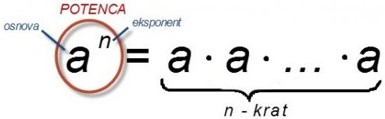
\includegraphics[scale=0.5]{Slike in skice/Potenca.jpg}
    %         \end{figure}
    
    %         \textbf{Pravila za računanje s potencami}:
    %         \begin{itemize}
    %             \item $\mathbf{a^n \cdot b^n = (ab)^n}$ - potenci z enakima eksponentoma zmnožimo tako, da zmnožimo osnovi in prepišemo eksponent
    %             \item $\mathbf{a^m \cdot a^n = a^{m+n}}$ - potenci z enako osnovo zmnožimo tako, da osnovo prepišemo in seštejemo eksponenta
    %             \item $\mathbf{(a^n)^m = a^{nm}}$ - potenco potenciramo tako, da osnovo prepišemo in zmnožimo eksponenta
    %         \end{itemize}

    %     \end{frame}

    % \subsection{Razčlenjevanje izrazov}

    %     \begin{frame}
    %         \frametitle{Razčlenjevanje izrazov}
    %     \end{frame}

    % \subsection{Razstavljanje izrazov v množici $\mathbb{Z}$}

    %     \begin{frame}
    %         \frametitle{Razstavljanje izrazov v množici $\mathbb{Z}$}
    %     \end{frame}

    % \subsection{Reševanje linearnih in razcepnih enačb v množici $\mathbb{Z}$}

    %     \begin{frame}
    %         \frametitle{Reševanje linearnih in razcepnih enačb v množici $\mathbb{Z}$}
    %     \end{frame}

    % \subsection{Reševanje linearnih neenačb v množici $\mathbb{Z}$}

    %     \begin{frame}
    %         \frametitle{Reševanje linearnih neenačb v množici $\mathbb{Z}$}
    %     \end{frame}


\section{Deljivost, izjave, množice}

\begin{frame}
    \sectionpage
\end{frame}

\begin{frame}
    \tableofcontents[currentsection, hideothersubsections]
\end{frame}

    \subsection{Relacija deljivosti}

        \begin{frame}
            \frametitle{Relacija deljivosti}
        \end{frame}

    \subsection{Pravila za deljivost}

        \begin{frame}
            \frametitle{Pravila za deljivost}
        \end{frame}

    \subsection{Praštevila in sestavljena števila}

        \begin{frame}
            \frametitle{Praštevila in sestavljena števila}
        \end{frame}

    \subsection{Največji skupni delitelj in najmanjši skupni večkratnik}

        \begin{frame}
            \frametitle{Največji skupni delitelj in najmanjši skupni večkratnik}
        \end{frame}

    \subsection{Osnovni izrek o deljenju}

        \begin{frame}
            \frametitle{Osnovni izrek o deljenju}
        \end{frame}

    \subsection{Evklidov algoritem in zveza $D v=ab$}

        \begin{frame}
            \frametitle{Evklidov algoritem in zveza $Dv=ab$}
        \end{frame}

    \subsection{Številski sestavi}

        \begin{frame}
            \frametitle{Številski sestavi}
        \end{frame}

    \subsection{Izjave}

        \begin{frame}
            \frametitle{Izjave}
        \end{frame}
        
    \subsection{Množice}

        \begin{frame}
            \frametitle{Množice}
        \end{frame}

\section{Racionalna števila}

\begin{frame}
    \sectionpage

\end{frame}

\begin{frame}
    \tableofcontents[currentsection, hideothersubsections]
\end{frame}

    \subsection{Ulomki in racionalna števila}

        \begin{frame}
            \frametitle{Ulomki}

            \begin{alertblock}{}
                \textbf{Ulomek} $\frac{x}{y}$ je zapis, ki predstavlja zapis deljenja $$x:y=\frac{x}{y};\quad y\neq 0\land x,y\in\mathbb{Z}.$$
                Število/izraz $x$ imenujemo \textbf{števec}, $y$ pa \textbf{imenovalec}, med njima je \textbf{ulomkova črta}.
            \end{alertblock}

            \begin{block}{}
                Ulomek $\frac{x}{0}$ ni definiran (nima pomena), saj z $0$ ne moremo deliti.
            \end{block}

            \begin{alertblock}{}
                \textbf{Algebrski ulomek} je ulomek, v katerem v števcu in/ali imenovalcu nastopajo algebrski izrazi.
            \end{alertblock}

        \end{frame}

        \begin{frame}

            \begin{block}{}
                Vsako celo število $x\in\mathbb{Z}$ lahko zapišemo z ulomkom: $x=\frac{x}{1}$.
            \end{block}

            \begin{block}{}
                \textbf{Ničelni ulomek} je ulomek oblike $\frac{0}{y}=0; y\neq 0$.
            \end{block}

            \begin{block}{}
                V ulomku, kjer v števcu ali imenovalcu nastopa negativno število, upoštevamo enakost $$-\frac{x}{y}=\frac{-x}{y}=\frac{x}{-y}.$$
            \end{block}

            \begin{alertblock}{}
                Vsakemu neničelnemu ulomku $\frac{x}{y}$ lahko priredimo njegovo \textbf{obratno vrednost}: $$\left(\frac{x}{y}\right)^{-1}=\frac{y}{x}; \quad x,y\in\mathbb{Z}\setminus\{0\}.$$
            \end{alertblock}

        \end{frame}


        \begin{frame}
            \frametitle{Racionalna števila}

            \begin{block}{}
                Množica racionalnih števil $\mathbb{Q}$ je sestavljena iz vseh ulomkov (kar pomeni, da vsebuje tudi vsa naravna in cela števila).
            \end{block}

            \only<2->{\begin{block}{}
                \centering
                \begin{tikzpicture}
                    % \clip (0,0) rectangle (14.000000,10.000000);
                    {\footnotesize
                    
                    % Drawing segment A B
                    \draw [line width=0.016cm] (1.000000,1.500000) -- (4.460000,1.500000);%
                    \draw [line width=0.016cm] (4.540000,1.500000) -- (8.000000,1.500000);%
                    
                    % Marking point 0 by circle
                    \draw [line width=0.016cm] (4.500000,1.500000) circle (0.040000);%
                    \draw (4.500000,1.500000) node [anchor=south] { $0$ };%
                    
                    \only<6->{
                    % Changing color 255 0 0
                    \definecolor{r255g0b0}{rgb}{1.000000,0.000000,0.000000}%
                    \color{r255g0b0}% 
                    
                    % Marking point \mathbb{Q}^+
                    \draw (6.250000,1.500000) node [anchor=south] { $\mathbb{Q}^+$ };%
                    
                    % Drawing segment B 0
                    \draw [line width=0.016cm] (8.000000,1.500000) -- (4.540000,1.500000);%
                    }

                    \only<4->{
                    % Changing color 0 255 0
                    \definecolor{r0g255b0}{rgb}{0.000000,1.000000,0.000000}%
                    \color{r0g255b0}% 
                    
                    % Marking point \mathbb{Q}^-
                    \draw (2.750000,1.500000) node [anchor=south] { $\mathbb{Q}^-$ };%
                    
                    % Drawing segment A 0
                    \draw [line width=0.016cm] (1.000000,1.500000) -- (4.460000,1.500000);%
                    }

                    % Changing color 0 0 0
                    \definecolor{r0g0b0}{rgb}{0.000000,0.000000,0.000000}%
                    \color{r0g0b0}% 
                    
                    % Marking point \mathbb{Q}
                    \draw (1.500000,2.000000) node  { $\mathbb{Q}$ };%
                    \color{black}
                    }
                    \end{tikzpicture}
                    
            \end{block}}

            \only<3->{\begin{block}{}
                Glede na predznak razdelimo racionalna števila v tri množice:
                \begin{itemize}
                    \item<4-> \textcolor{green}{množico negativnih racionalnih števil $\mathbf{\mathbb{Q}^-}$},
                    \item<5-> množico z elementom nič: $\mathbf{\{0\}}$ in
                    \item<6-> \textcolor{red}{množico pozitivnih racionalnih števil: $\mathbf{\mathbb{Q}^+}$}.
                \end{itemize}
                $$ \mathbb{Q}=\only<4->{\textcolor{green}{\mathbb{Q}^-}}\only<5->{\cup\{0\}}\only<6->{\cup\textcolor{red}{\mathbb{Q}^+}} $$
            \end{block}}
            

            % \only<7->{\begin{block}{}
            %     Množica racionalnih števil je povsod gosta, saj lahko med poljubnima racionalnima številoma vedno najdemo racionalno število (posledično je med dvema racionalnima številoma neskončno mnogo racionalnih števil).
            % \end{block}}

        \end{frame}

        \begin{frame}
            \begin{block}{}
                Ulomka $\frac{x}{y}$ in $\frac{z}{w}$ sta enaka/enakovredna natanko takrat, ko je $xz=wy$; $y,z\neq 0$.
                $$\frac{x}{y}=\frac{w}{z}\Leftrightarrow xz=wy; \quad y,z\neq 0$$
            \end{block}

            \begin{block}{}
                Enaka/enakovredna ulomka sta različna zapisa za isto racionalno število.
            \end{block}
        \end{frame}


        \begin{frame}
            \only<2->{\begin{exampleblock}{Naloga}
                Za katere vrednosti $x$ ulomek ni definiran?
                \only<3->{\begin{itemize}
                    \item $\frac{x-2}{x+1}$ \\~
                    \item $\frac{2}{x-5}$ \\~
                    \item $\frac{x+2}{3}$ \\~
                    \item $\frac{13}{2x-5}$ \\~
                \end{itemize}}
            \end{exampleblock}}
        \end{frame}

        \begin{frame}
            \only<2->{\begin{exampleblock}{Naloga}
                Za katere vrednosti $x$ ima ulomek vrednost enako $0$?
                \only<3->{\begin{itemize}
                    \item $\frac{x-2}{x+1}$ \\~
                    \item $\frac{2}{x-5}$ \\~
                    \item $\frac{x+2}{3}$ \\~
                    \item $\frac{13}{2x-5}$ \\~
                \end{itemize}}
            \end{exampleblock}}
        \end{frame}

        \begin{frame}
            \only<2->{\begin{exampleblock}{Naloga}
                Ali imata ulomka isto vrednost?
                \only<3->{\begin{itemize}
                    \item $\frac{2}{3}$ in $\frac{10}{15}$ \\~
                    \item $\frac{-1}{2}$ in $\frac{1}{-2}$ \\~
                    \item $\frac{4}{5}$ in $\frac{-8}{-10}$ \\~
                    \item $\frac{5}{8}$ in $\frac{8}{5}$ \\~
                \end{itemize}}
            \end{exampleblock}}
        \end{frame}

        \begin{frame}
            \only<2->{\begin{exampleblock}{Naloga}
                Za kateri $x$ imata ulomka isto vrednost?
                \only<3->{\begin{itemize}
                    \item $\frac{x+1}{2}$ in $\frac{3}{4}$ \\~
                    \item $\frac{4}{2x-1}$ in $\frac{1}{3}$ \\~
                    \item $\frac{x+1}{2}$ in $\frac{x-1}{-3}$ \\~
                    \item $\frac{x+1}{x-2}$ in $\frac{2}{5}$ \\~
                \end{itemize}}
            \end{exampleblock}}
        \end{frame}

        \begin{frame}
            \only<2->{\begin{exampleblock}{Naloga}
                Ali ulomka predstavljata isto vrednost?
                \only<3->{\begin{itemize}
                    \item $\left(\frac{1}{2}\right)^{-1}$ in $-\frac{1}{2}$ \\~\\~
                    \item $\left(\frac{2}{3}\right)^{-1}$ in $\frac{3}{2}$ \\~\\~
                    \item $1\frac{3}{7}$ in $\left(\frac{7}{10}\right)^{-1}$ \\~\\~
               \end{itemize}}
            \end{exampleblock}}
        \end{frame}

        \begin{frame}
            \only<2->{\begin{exampleblock}{Naloga}
                Ali ulomka predstavljata isto vrednost?
                \only<3->{\begin{itemize}
                    \item $2\cdot\frac{3}{4}$ in $\frac{3}{2}$ \\~
                    \item $2\frac{3}{4}$ in $\frac{3}{2}$ \\~
                    \item $\left(1\frac{2}{5}\right)^{-1}$ in $1\frac{5}{2}$ \\~
                    \item $\left(1\frac{2}{5}\right)^{-1}$ in $\frac{5}{7}$ \\~
               \end{itemize}}
            \end{exampleblock}}
        \end{frame}

        \begin{frame}
            \only<2->{\begin{exampleblock}{Naloga}
                Zapišite s celim delom oziroma z ulomkom.
                \only<3->{\begin{itemize}
                    \item $\frac{14}{5}$ \\~
                    \item $-\frac{5}{2}$ \\~
                    \item $\frac{4}{3}$ \\~
                    \item $\frac{110}{17}$ \\~
                    \item $3\frac{5}{8}$ \\~
                    \item $2\frac{9}{2}$ \\~
               \end{itemize}}
            \end{exampleblock}}
        \end{frame}

        % \begin{frame}
        %     \only<2->{\begin{exampleblock}{Naloga}
        %         Poenostavite.
        %         \only<3->{\begin{itemize}
        %             \item a \\~
        %         \end{itemize}}
        %     \end{exampleblock}}
        % \end{frame}

        % \begin{frame}
        %     \only<2->{\begin{exampleblock}{Naloga}
        %         Poenostavite.
        %         \only<3->{\begin{itemize}
        %             \item a \\~
        %         \end{itemize}}
        %     \end{exampleblock}}
        % \end{frame}




        \subsection{Urejenost racionalnih števil}
        \begin{frame}
            \frametitle{Urejenost racionalnih števil}

            \only<2->{\begin{alertblock}{}
                Množica racionalnih števil je \textbf{linearno urejena} z relacijo \textit{biti manjši} ($<$) oziroma \textit{biti večji} ($>$). Za ulomka $\frac{a}{b}$ in $\frac{c}{d}$ ($b,d\in\mathbb{N}$) velja natanko ena izmed treh možnosti:
                \begin{enumerate}
                    \item<3-> prvi ulomek je večji od drugega $\frac{a}{b}>\frac{c}{d}$ natanko tedaj, ko je $ad>bc$;
                    \item<4-> drugi ulomek je večji od prvega $\frac{a}{b}<\frac{c}{d}$ natanko tedaj, ko je $ad<bc$;
                    \item<5-> ulomka sta enaka $\frac{a}{b}=\frac{c}{d}$ natanko tedaj, ko je $ad=bc$.
                \end{enumerate}
            \end{alertblock}}


            \only<6->{\begin{block}{}
                Enaka ulomka predstavljata isto racionalno število.
            \end{block}}

        \end{frame}



        \begin{frame}
            \only<2->{\begin{block}{}
                Slika večjega racionalnega števila \textcolor{red}{$\frac{a}{b}$} je na številski premici desno od slike manjšega racionalnega števila \textcolor{green}{$\frac{c}{d}$}. \\
                \only<3->{\centering
                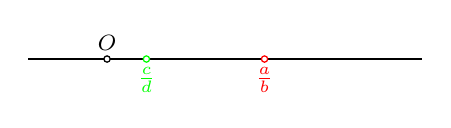
\begin{tikzpicture}
                    % \clip (0,0) rectangle (14.000000,10.000000);
                    {\footnotesize
                    
                    % Drawing segment A B
                    \draw [line width=0.016cm] (1.000000,1.500000) -- (1.960000,1.500000);%
                    \draw [line width=0.016cm] (2.040000,1.500000) -- (2.460000,1.500000);%
                    \draw [line width=0.016cm] (2.540000,1.500000) -- (3.960000,1.500000);%
                    \draw [line width=0.016cm] (4.040000,1.500000) -- (6.000000,1.500000);%
                    
                    % Marking point O by circle
                    \draw [line width=0.016cm] (2.000000,1.500000) circle (0.040000);%
                    \draw (2.000000,1.500000) node [anchor=south] { $O$ };%
                    
                    % Changing color 255 0 0
                    \definecolor{r255g0b0}{rgb}{1.000000,0.000000,0.000000}%
                    \color{r255g0b0}% 
                    
                    % Marking point \frac{a}{b} by circle
                    \draw [line width=0.016cm] (4.000000,1.500000) circle (0.040000);%
                    \draw (4.000000,1.500000) node [anchor=north] { $\frac{a}{b}$ };%
                    
                    % Changing color 0 255 0
                    \definecolor{r0g255b0}{rgb}{0.000000,1.000000,0.000000}%
                    \color{r0g255b0}% 
                    
                    % Marking point \frac{c}{d} by circle
                    \draw [line width=0.016cm] (2.500000,1.500000) circle (0.040000);%
                    \draw (2.500000,1.500000) node [anchor=north] { $\frac{c}{d}$ };%
                    \color{black}
                    }
                \end{tikzpicture}}    
            \end{block}}

            \only<4->{\begin{block}{}
                Slike pozitivnih racionalnih števil ležijo desno, slike negativnih racionalnih števil pa levo od koordinatnega izhodišča. \\
                \only<5->{\centering
                \begin{tikzpicture}
                    
                    % \clip (0,0) rectangle (14.000000,10.000000);
                    {\footnotesize
                    
                    % Drawing segment A B
                    \draw [line width=0.016cm] (1.000000,1.500000) -- (3.460000,1.500000);%
                    \draw [line width=0.016cm] (3.540000,1.500000) -- (6.000000,1.500000);%
                    
                    % Changing color 255 0 0
                    \definecolor{r255g0b0}{rgb}{1.000000,0.000000,0.000000}%
                    \color{r255g0b0}% 
                    
                    % Drawing segment B O
                    \draw [line width=0.016cm] (6.000000,1.500000) -- (3.540000,1.500000);%
                    
                    % Marking point pozitivna_tevila
                    \draw (4.750000,1.500000) node [anchor=north] { $pozitivna~ števila$ };%
                    \draw (4.750000,1.500000) node [anchor=south] { $\mathbb{Q}^+$ };%
                    
                    % Changing color 0 255 0
                    \definecolor{r0g255b0}{rgb}{0.000000,1.000000,0.000000}%
                    \color{r0g255b0}% 
                    
                    % Drawing segment O A
                    \draw [line width=0.016cm] (3.460000,1.500000) -- (1.000000,1.500000);%
                    
                    % Marking point negativna_tevila
                    \draw (2.250000,1.500000) node [anchor=north] { $negativna~ števila$ };%
                    \draw (2.250000,1.500000) node [anchor=south] { $\mathbb{Q}^-$ };%
                    
                    % Changing color 0 0 0
                    \definecolor{r0g0b0}{rgb}{0.000000,0.000000,0.000000}%
                    \color{r0g0b0}% 
                    
                    % Marking point O by circle
                    \draw [line width=0.032cm] (3.500000,1.500000) circle (0.040000);%
                    \draw (3.500000,1.500000) node [anchor=south] { $O$ };%
                    \color{black}
                    }
                \end{tikzpicture}}
            \end{block}}

            \only<6->{\begin{block}{}
                V množici ulomkov velja, da je vsak negativen ulomek manjši od vsakega pozitivnega ulomka.
            \end{block}}

        \end{frame}

        \begin{frame}
            \frametitle{Lastnosti relacije urejenosti}
            
            \only<2->{\begin{alertblock}{Monotonost vsote}
                \only<3->{Če na obeh straneh neenakosti prištejemo isto število, se neenakost ohrani.}
                \only<4->{$$ \mathbf{\frac{a}{b}<\frac{c}{d} \quad \Rightarrow \quad \frac{a}{b}+\frac{e}{f}<\frac{c}{d}+\frac{e}{f}} $$}
                % \only<5->{$$ \mathbf{p<q \quad \Rightarrow \quad p+r<q+r} $$}
            \end{alertblock}}

            \only<6->{\begin{alertblock}{Tranzitivnost}
                \only<7->{$$ \mathbf{\frac{a}{b}<\frac{c}{d} \quad \wedge \quad \frac{c}{d}<\frac{e}{f} \quad \Rightarrow \quad \frac{a}{b}<\frac{e}{f}} $$}
                % \only<8->{$$ \mathbf{p<q \quad \wedge \quad q<r \quad \Rightarrow \quad p<r} $$}
            \end{alertblock}}

        \end{frame}

        \begin{frame}

            \only<2->{\begin{alertblock}{}
                Pri množenju neenakosti s pozitivnim številom se znak neenakosti ohrani.
                \only<3->{$$ \mathbf{\frac{a}{b}<\frac{c}{d} \quad \wedge \quad \frac{e}{f}>0 \quad \Rightarrow \quad \frac{a}{b}\cdot\frac{e}{f}<\frac{c}{d}\cdot\frac{e}{f}} $$}
                % \only<4->{$$ \mathbf{p<q \quad \wedge \quad r>0 \quad \Rightarrow \quad p\cdot r<q\cdot r} $$}
            \end{alertblock}}

            \only<5->{\begin{alertblock}{}
                Pri množenju neenakosti s negativnim številom se znak neenakosti obrne.
                \only<6->{$$ \mathbf{\frac{a}{b}<\frac{c}{d} \quad \wedge \quad \frac{e}{f}<0 \quad \Rightarrow \quad \frac{a}{b}\cdot\frac{e}{f}>\frac{c}{d}\cdot\frac{e}{f}} $$}
                % \only<7->{$$ \mathbf{p<q \quad \wedge \quad r>0 \quad \Rightarrow \quad p\cdot r>q\cdot r} $$}
            \end{alertblock}}

            \only<8->{\begin{block}{}
                Pri prehodu na nasprotno vrednost se neenačaj obrne:
                \only<9->{$$ \mathbf{\frac{a}{b}<\frac{c}{d} \quad \Rightarrow \quad -\frac{a}{b}>-\frac{c}{d}} $$}
            \end{block}}



        \end{frame}

        \begin{frame}
            
            \only<2->{\begin{alertblock}{}
                Množica racionalnih števil pa je tudi \textbf{delno urejena}, in sicer z relacijo \textit{biti manjši ali enak} ($\leq$) oziroma \textit{biti večji ali enak} ($\geq$). Za ulomka $\frac{a}{b}$ in $\frac{c}{d}$ ($b,d\in\mathbb{N}$) velja vsaj ena izmed možnosti:
                \begin{enumerate}
                    \item<3-> prvi ulomek je večji ali enak od drugega $\frac{a}{b}\geq\frac{c}{d}$ natanko tedaj, ko je $ad\geq bc$;
                    \item<4-> drugi ulomek je večji ali enak od prvega $\frac{a}{b}\geq\frac{c}{d}$ natanko tedaj, ko je $ad\leq bc$;
                \end{enumerate}
            \end{alertblock}}

            \only<5->{\begin{block}{}
                Za (zgornjo) relacijo delne urejenosti veljajo naslednje lastnosti:
                \begin{itemize}
                    \item<6-> $\frac{a}{b}\leq\frac{a}{b}$ -- \textbf{refleksivnost};
                    \item<7-> $\frac{a}{b}\leq\frac{c}{d}  \wedge \frac{c}{d}\leq\frac{a}{b} \Rightarrow \frac{a}{b}=\frac{c}{d}$ -- \textbf{antisimetričnost} in
                    \item<8-> $\frac{a}{b}\leq\frac{c}{d}  \wedge \frac{c}{d}\leq\frac{e}{f} \Rightarrow \frac{a}{b}\leq\frac{e}{f}$ -- \textbf{tranzitivnost}.
                \end{itemize}
            \end{block}}


        \end{frame}

    \subsection{Algebrski ulomki}

        \begin{frame}
            \frametitle{Algebrski ulomki}
        \end{frame}

    \subsection{Računanje z ulomki}

        \begin{frame}
            \frametitle{Računanje z ulomki}
        \end{frame}

    \subsection{Potence s celimi eksponenti}

        \begin{frame}
            \frametitle{Potence s celimi eksponenti}
        \end{frame}

    \subsection{Pravila za računanje s potencami s celimi eksponenti}

        \begin{frame}
            \frametitle{Pravila za računanje s celimi eksponenti}
        \end{frame}

    \subsection{Premo in obratno sorazmerje}

        \begin{frame}
            \frametitle{Premo in obratno sorazmerje}
        \end{frame}

    \subsection{Odstotki}

        \begin{frame}
            \frametitle{Odstotki}
        \end{frame}


\section{Realna števila, statistika}

\begin{frame}
    \sectionpage
\end{frame}

\begin{frame}
    \tableofcontents[currentsection, hideothersubsections]
\end{frame}

    \subsection{Realna števila}

        \begin{frame}
            \frametitle{Realna števila}
        \end{frame}

    \subsection{Kvadratni in kubični koren}

        \begin{frame}
            \frametitle{Kvadratni in kubični koren}
        \end{frame}

    \subsection{Intervali}

        \begin{frame}
            \frametitle{Intervali}
        \end{frame}

    \subsection{Absolutna vrednost}

        \begin{frame}
            \frametitle{Absolutna vrednost}
        \end{frame}

    \subsection{Sistem linearnih enačb}

        \begin{frame}
            \frametitle{Sistem linearnih enačb}
        \end{frame}

    \subsection{Obravnavanje linearnih enačb, neenačb, sistemov}

        \begin{frame}
            \frametitle{Obravnavanje linearnih enačb, neenačb, sistemov}
        \end{frame}

    \subsection{Absolutna in relativna napaka}

        \begin{frame}
            \frametitle{Absolutna in relativna napaka}
        \end{frame}

    \subsection{Sredine}

        \begin{frame}
            \frametitle{Sredine}
        \end{frame}

    \subsection{Razpršenost podatkov}

        \begin{frame}
            \frametitle{Razpršenost podatkov}
        \end{frame}

    \subsection{Prikazi}
        
        \begin{frame}
            \frametitle{Prikazi}
        \end{frame}

\section{Pravokotni koordinatni sistem, linearna funkcija}

\begin{frame}
    \sectionpage
\end{frame}

\begin{frame}
    \tableofcontents[currentsection, hideothersubsections]
\end{frame}

    \subsection{Pravokotni koordinatni sistem}

        \begin{frame}
            \frametitle{Pravokotni koordinatni sistem}
        \end{frame}

    \subsection{Razdalja med točkama in razpolovišče daljice}

        \begin{frame}
            \frametitle{Razdalja med točkama in razpolovišče daljice}
        \end{frame}

    \subsection{Ploščina trikotnika}

        \begin{frame}
            \frametitle{Ploščina trikotnika}
        \end{frame}

    \subsection{Osnovno o funkcijah}

        \begin{frame}
            \frametitle{Osnovno o funkcijah}
        \end{frame}

    \subsection{Linearna funkcija in premica}

        \begin{frame}
            \frametitle{Linearna funkcija in premica}
        \end{frame}

    \subsection{Oblike enačbe premice}

        \begin{frame}
            \frametitle{Oblike enačbe premice}
        \end{frame}

    \subsection{Presešišče premic}

        \begin{frame}
            \frametitle{Presešišče premic}
        \end{frame}

    \subsection{Sistem linearnih neenačb}

        \begin{frame}
            \frametitle{Sistem linearnih neenačb}
        \end{frame}

    \subsection{Modeliranje z linearno funkcijo}

        \begin{frame}
            \frametitle{Modeliranje z linearno funkcijo}
        \end{frame}

    \subsection{(i) Linearno programiranje}
        
        \begin{frame}
            \frametitle{(i) Linearno programiranje}
        \end{frame}



\end{document}